\chapter{Goby MOOS Modules}\label{chap:MOOS}
\MakeShortVerb{\!} % makes !foo! == !foo!

The acoustic communications portion of Goby was developed originally for the MOOS autonomy architecture. Thus, the relevant MOOS modules !pAcommsHandler! and others are still maintained (in goby/src/moos) for the use of the !MOOS-IvP! community. !MOOS-IvP! is explained in \cite{moos-ivp-jfr} and is available at \url{http://moos-ivp.org}. The usage of these modules is documented here. See \url{http://gobysoft.org/wiki/InstallingGoby} for how to install Goby.


\section{Goby MOOS Applications} \label{sec:goby_moos_app}

The Goby MOOS applications share a common subclass of CMOOSApp that provides a validating configuration reader based on the Google Protocol Buffers TextFormat class. The configuration is still embedded within the .moos file, but the syntax is somewhat different. Here you can control logging to a text file and terminal verbosity. You can also initialize a variable in the MOOS database at startup. Many of these parameters will automatically be set to a global MOOS variable (specified outside any ProcessConfig block) if left empty. For example, the global MOOS variable !LatOrigin! will set the Goby MOOS configuration variable !common::lat_origin!. This allows Goby MOOS applications to conform to MOOS \textit{de facto} conventions.

Any Goby MOOS application will give all its valid configuration parameters with \begin{verbatim}
> pGobyApp --example_config
\end{verbatim} 

\boxedverbatiminput{@RELATIVE_CMAKE_CURRENT_SOURCE_DIR@/includes/common.pb.cfg}
\resetbvlinenumber

Some details about the configuration values:

\begin{itemize}
\item !log!: boolean to indicate whether to log terminal output or not to files in the path by !log_path!.
\item !log_path!: folder to log all terminal output to for later debugging. Similar to system logs in /var/log.
\item !log_verbosity!: verbosity of the log file. See !verbosity! for the various settings.
\item !community!: the name of the current vehicle community. If omitted, read from the !Community=! global MOOS configuration field.
\item !lat_origin!: a decimal degrees latitude indicating the local cartesian origin. If omitted, read from the !LatOrigin=! global MOOS configuration field.
\item !lon_origin!: a decimal degrees longitude indicating the local cartesian origin. If omitted, read from the !LongOrigin=! global MOOS configuration field.
\item !app_tick!: same as AppTick.
\item !comm_tick!: same as CommsTick.
\item !verbosity!: choose !DEBUG1!-!DEBUG3! for various levels of debugging output, !VERBOSE! for some text terminal output, !WARN! for warnings only, and !QUIET! for no terminal output.
\item !show_gui!: if true, the running terminal opens an NCurses GUI helpful to debugging and visualizing the many data flows of pAcommsHandler. The verbosity in this GUI is governed by !verbosity!.
\item !initializer!: since many times it is useful to have a MOOS variable including in a message that remains static for a given mission (vehicle name, etc), we give the option to publish initial MOOS variables here (for later use in messages [until overwritten, of course]). If !global_cfg_var! is set, pAcommsHandler looks for a global (i.e. specified at the top of the MOOS file or outside any !ProcessConfig! blocks) value in the .moos file with the name to the right of the colon and publishes it to a MOOS variable with the name to the left of the colon. For example:
\begin{verbatim}
initializer { global_cfg_var: "LatOrigin" moos_var: "LAT_ORIGIN" } 
\end{verbatim}
\resetbvlinenumber
looks for a variable in the .moos file called !LatOrigin! and publishes it to the MOOSDB as a double variable !LAT_ORIGIN! with the value given by !LatOrigin!.
\end{itemize}


\section{pTranslator}
\label{sec:ptranslator} 

!pTranslator! is a translator between MOOS types (strings and doubles) and Google Protocol Buffers messages (which includes DCCL messages). All of the functionality of !pTranslator! is also present in !pAcommsHandler!, but !pTranslator! is provided as a standalone application for cases when Goby-Acomms is not needed, but the translation functionality is. Also, pTranslator loops back all created messages and immediately publishes them, whereas pAcommsHandler publishes messages received acoustically, and creates messages to be transmitted.

The configuration for !pTranslator! is as follows:

\boxedverbatiminput{@RELATIVE_CMAKE_CURRENT_SOURCE_DIR@/includes/pTranslator.moos}
\resetbvlinenumber

\begin{itemize}
\item !common!: Parameters that can be set for any of the Goby MOOS applications. See section \ref{sec:goby_moos_app}.
\item !load_shared_library!: Repeated string, each with a path to a shared library containing compiled DCCL (Google Protocol Buffers) messages.
\item !load_proto_file!: Repeated string, each with one path to a .proto file containing compiled DCCL (Google Protocol Buffers) messages. These will be compiled at runtime and loaded. It is preferable to use !load_shared_library! when possible, as syntactical and type mistakes in the DCCL messages will be caught at compile-time rather than delayed to runtime.
\item !translator_entry!: Repeated entry: there should be one !translator_entry! defined for each Google Protobuf message type that you wish to translate to or from.
\begin{itemize}
\item !protobuf_name!: Fully qualified name (packages separated by !.!, e.g. !example.MinimalStatus!) to the Protobuf message that this translator should use. This message must be loaded either by !load_shared_library! or !load_proto_file!. 
\item !trigger!: The event that causes this translation to occur.
\begin{itemize}
\item !type!: Either !TRIGGER_PUBLISH! (do a translation every time a given MOOS variable is published to) or !TRIGGER_TIME! (do a translation on a regular frequency).
\item !moos_var!: For !TRIGGER_PUBLISH!, the MOOS variable that causes the translation to occur.
\item !period!: For !TRIGGER_TIME!, the period (in seconds) between translations.
\item !mandatory_content!: For !TRIGGER_PUBLISH!, if this is defined, the !moos_var! must contain this substring in order to trigger this translation. Use of this field allows a single MOOS variable to trigger several different translations.
\end{itemize}
\item !create!: Upon triggering, this defines how the Protobuf message is created from one or more MOOS variables. Repeat this field for multiple MOOS variables. The !create! directives are processed in the order they are defined and thus later !create!s that write the same fields will overwrite earlier ones.
\begin{itemize}
\item !technique!: The parsing technique to use. See section \ref{sec:ptranslator_techniques}.
\item !moos_var!: The MOOS variable to use for this !create!. 
\item !format!: For !TECHNIQUE_FORMAT!, the format string to use. This is similar to scanf, but instead of type specifiers, numerical specifiers are used, surrounded by !%! on both sides. For example, if the !format! value is !foo=%1%!, this !create! will parse a !moos_var! containing !foo=5! and put the value !5! into field 1 of the Protobuf message given by !protobuf_name!. %
\item !repeated_delimiter!: When parsing for !repeated! Protobuf fields, this is the string that delimits fields. For example, if !foo=%1%!, field 1 is !repeated int32 field_name = 1!, and the value to parse is !foo=10;12;13;14!, !repeated_delimiter! should be ``;'' in order to parse these four numbers into a ``vector'' of values in that field. %
\item !algorithm!: An algorithm to modify the parsed field before placing it in the Protobuf message. These are largely provided for backwards compatibility for Goby v1, and are not necessarily encouraged for new use. See \url{http://gobysoft.com/dl/goby1-user-manual.pdf} for a detailing of the available algorithms. Several algorithms can be chained (processed in the order they are defined) by repeated this !algorithm! field with the same !primary_field!.
\begin{itemize}
\item !name!: Name of the algorithm, e.g. !to_upper!.
\item !primary_field!: The field number to apply this algorithm to. 
\end{itemize}
\end{itemize}
\item !publish!: Upon receipt of a Protobuf message, how to publish it back to one or more MOOS variable(s). Several !publish! entries should be specified to publish to several MOOS variables.
\begin{itemize}
\item !technique!: The serialization technique to use. See section \ref{sec:ptranslator_techniques}.
\item !moos_var!: The MOOS variable to write to for this !publish!. 
\item !format!: For !TECHNIQUE_FORMAT!, the format string to use. This is similar to printf, but instead of type specifiers, numerical specifiers are used, surrounded by !%! on both sides. For example, if the !format! value is !foo=%1%!, this !publish! will write a !moos_var! containing !foo=5! if field 1 in the Protobuf message was !5!. %
\item !repeated_delimiter!: When writing !repeated! Protobuf fields, this is the string that is used to delimit fields. 
\item !algorithm!: Several algorithms can be chained (processed in the order they are defined) by repeated this !algorithm! field with the same !primary_field!.
\begin{itemize}
\item !name!: Name of the algorithm, e.g. !to_upper!.
\item !primary_field!: The field number to apply this algorithm to. 
\item !output_virtual_field!: A ``virtual'' field number (one that doesn't exist in the actual Protobuf message) that is used to specify the output of this algorithm. This virtual field can then be used in the !format! string like a real field. 
\item !reference_field!: The field(s) required by the algorithm as references, if the algorithm requires them (e.g. !utm_x2lon!).
\end{itemize}
\end{itemize}
\item !use_short_enum!: If true, the front of the enumeration value is removed if it matches the field name plus a !_!. For example, if the enum field is !foo!, and the enumerations are !FOO_OPTION1!, !FOO_OPTION2!, then !OPTION1! and !OPTION2! are published. If false (the default), the enumeration values are published as defined. This is mostly here for backwards compatibility with Goby 1.
\end{itemize}
\end{itemize}


\section{Translator techniques}
\label{sec:ptranslator_techniques} 

There are three broad categories of translator techniques: 1) those that use the Google Protocol Buffers tools (!TECHNIQUE_PREFIXED_PROTOBUF_TEXT_FORMAT!, \\ !TECHNIQUE_PROTOBUF_TEXT_FORMAT!, !TECHNIQUE_PROTOBUF_NATIVE_ENCODED!), 2) one that uses the \textit{de facto} MOOS convention of !key=value! pairs delimited by commas \\(!TECHNIQUE_COMMA_SEPARATED_KEY_EQUALS_VALUE_PAIRS!), and 3) one that is based roughly on printf/scanf (!TECHNIQUE_FORMAT!).

More details on each translator type:
\begin{itemize}
\item !TECHNIQUE_PROTOBUF_TEXT_FORMAT!: exactly the same as if you used the Google TextFormat class: \url{https://developers.google.com/protocol-buffers/docs/reference/cpp/google.protobuf.text_format}.
\item !TECHNIQUE_PREFIXED_PROTOBUF_TEXT_FORMAT! (recommendated for most uses). Same as !TECHNIQUE_PROTOBUF_TEXT_FORMAT! but prefixed with !@PB[TypeName] !, so that you can put multiple Protobuf Types in a single MOOS Variable (if you really need to). It's also quite human readable and allows for programs to read / write generic Protobuf messages. This technique is useful enough, there are two shortcut functions for use in your C++ MOOS code\\(!#include "goby/moos/moos_protobuf_helpers.h"!): !serialize_for_moos! and \\!parse_for_moos!.
\item !TECHNIQUE_PROTOBUF_NATIVE_ENCODED!: exactly the same as if you used the default binary Google encoding (binary), represented as a byte string. This tends to break the MOOS tools that assume strings are ASCII / UTF-8. 
\item !TECHNIQUE_COMMA_SEPARATED_KEY_EQUALS_VALUE_PAIRS!: all fields represented as !key1=value1,key2=value2,...! Messages with submessages are flattened and the keys assembled by concatenation separated with !_!. This is similar to the existing !NODE_REPORT! variable used in MOOS-IvP.
\item !TECHNIQUE_FORMAT!: sort of like !printf! / !scanf!, except instead of typed directives (e.g. !%d!), Goby uses numeric directives that correspond the protobuf message field id (e.g. !foobar=%2%!). Submessages can be referenced using ``:'' (e.g. !%5:1%!, where field 5 is a Message), repeated fields can be referenced using ``.'' (e.g. !%7.1%!, where field 7 is repeated). Note the ending !%! on each directive, which is different than !printf!. 
\end{itemize}

\section{pAcommsHandler}
\label{sec:pacommshandler} 

pAcommsHandler provides a:
\begin{enumerate}
\item MOOS Application wrapper for the Goby-Acomms communication library.
\item set of translation tools for converting the DCCL messages (written as an extension of Google Protocol Buffers) to MOOS types (strings and doubles) and vice-versa.
\item full backwards-compatibility support module for version 1 XML messages. 
\end{enumerate}

This section describes only the parts relevant for interface to MOOS (variables and translator entries that allow you to read and write to and from DCCL (Protobuf) messages). You should read Chapter \ref{chap:acomms} before starting this section and reference it as necessary.

\subsection{Parameters for the pAcommsHandler Configuration Block}\label{sec:pAcommsHandler:config}

\subsubsection{Example moos file}

pAcommsHandler has a large number of configuration options, many of which you will never use or leave as default. You can always get a complete listing of MOOS file parameters with their syntax by running
\begin{verbatim}
> pAcommsHandler --example_config
\end{verbatim}
\resetbvlinenumber

These configuration values are provided here (with $\ldots$ where the relevant configuration is provided elsewhere in this document):

\boxedverbatiminput{@RELATIVE_CMAKE_CURRENT_SOURCE_DIR@/includes/pAcommsHandler_reduced.moos}
\resetbvlinenumber


\subsubsection{Filling out the .moos file}\label{sec:pAcommsHandler_moos_file}

Many of the parameters are sufficiently explained in the above list of configuration parameters. What follows is a detailed explanation of the parameters that need further explanation.

\begin{itemize}
\item !common!: Parameters that can be set for any of the Goby MOOS applications. See section \ref{sec:goby_moos_app}.
\item !modem_id!: integer that specifies the !modem_id! of this current vehicle / community. For the WHOI Micro-Modem this is the Micro-Modem ``SRC'' configuration parameter (as set by !$CCCFG,SRC,#!). For the remainder of the document, !modem_id! refers to the value !$CCCFG,SRC,modem_id!. This configuration parameter will be set on startup. Setting this within the main block for pAcommsHandler sets it for all the modules (!driver_cfg!, !queue_cfg!, !mac_cfg!) 
\item !driver_type!: 
\begin{itemize}
\item !DRIVER_WHOI_MICROMODEM! is a driver for the WHOI Micro-Modem. 
\item !DRIVER_ABC_EXAMPLE_MODEM! is a simple test ``modem''. Do not use this for real work, but rather for learning how to write new drivers for Goby.
\item !DRIVER_UFIELD_SIM_DRIVER! is a driver for the MOOS-IvP uField toolbox.
\item !DRIVER_PB_STORE_SERVER! is a ZeroMQ (TCP, UNIX sockets) driver for the !goby_store_server! database.
\item !DRIVER_UDP! is a user datagram protocol (UDP) driver. This is probably the easiest driver to start with for learning pAcommsHandler.
\item !DRIVER_NONE! disables the modem driver.
\end{itemize}
\item !driver_cfg!: Configures the base driver and the specific driver selected. See section \ref{sec:driver}.
\item !mac_cfg!: Configures the acoustic Medium Access Control. See section \ref{sec:amac}.
\item !queue_cfg!: Configures the Priority Queuing layer. See section \ref{sec:queue}.
\item !dccl_cfg!: Configures the Dynamic Compact Control Language. See section \ref{sec:dccl}.
\item !route_cfg!: Configures a basic static routing module. This is experimental and subject to change.
\item !moos_var!: Rename any or all of the MOOS variables published by pAcommsHandler.
\item !load_shared_library!: Repeated string, each with a path to a shared library containing compiled DCCL (Google Protocol Buffers) messages.
\item !load_proto_file!: Repeated string, each with one path to a .proto file containing compiled DCCL (Google Protocol Buffers) messages. These will be compiled at runtime and loaded. It is preferable to use !load_shared_library! when possible, as syntactical and type mistakes in the DCCL messages will be caught at compile-time rather than delayed to runtime.
\item !translator_entry!: List of entries indicating when to make (\textit{trigger}) and how to \textit{create} outgoing DCCL messages, and how to \textit{publish} incoming DCCL messages. This can be thought of as providing a generic interface between MOOS strings and Google Protocol Buffers messages. See section \ref{sec:ptranslator} for a full explanation on how to configure this translation.
\item !multiplex_create_moos_var!: Used by !goby_liaison! to publish multiple commands (outgoing messages) on a single MOOS variable.
\item !modem_id_lookup_path!: path to a text file giving the mapping between !modem_id! and vehicle name and type for a given experiment. This file should look like:
\begin{boxedverbatim}
// modem id, vehicle name (should be community name), vehicle type
0, broadcast, broadcast
1, endeavor, ship
3, unicorn, auv
4, macrura, auv
\end{boxedverbatim}
\resetbvlinenumber
\item !transitional_cfg!: Provides the same functionality as !dccl_cfg! does in pAcommsHandler from version 1 of Goby. Behind the scenes, XML messages are read, translated to version 2 Protobuf DCCL messages, and written to the !generated_proto_dir!, and subsequently loaded using !load_proto_file!. The appropriate !translator_entry!s are also created from these messages. Do not use this configuration or the XML representation of DCCL messages for any new projects. See the version 1 documentation (\url{http://gobysoft.org/doc/1.1/}) for more details on the XML representation of DCCL messages.
\end{itemize}

%\subsection{MOOS variables subscribed to by pAcommsHandler}
%
%Except for the user-configured publishes (!translator_entry!), pAcommsHandler uses the \href{http://code.google.com/apis/protocolbuffers/docs/reference/cpp/google.protobuf.text_format.html}{Google Protocol Buffers TextFormat} class for serializing to and parsing from MOOS strings (same as !TECHNIQUE_PREFIXED_PROTOBUF_TEXT_FORMAT!). This saves significant effort in manually parsing strings. You should use these same facilities for creating and reading messages. Two helper functions are provided in \\ \href{http://gobysoft.com/doc/moos__protobuf__helpers_8h.html}{goby/moos/libmoos\_util/moos\_protobuf\_helpers} will help you serialize and parse these messages. See \url{http://gobysoft.com/doc/2.0/acomms.html#protobuf} for a brief overview of Google Protocol Buffers as used in Goby.
%
%\begin{itemize}
%\item !DCCL!: Most variables subscribed to by pAcommsHandler are configured in the message XML files and are designated by the tags \xmltag{src\_var} (used to fetch data for a particular !message_var! within a DCCL message) and \xmltag{trigger\_var} (used to trigger the creatinon of a particular DCCL message and possibly provide some data for that message. See \ref{sec:dccl_overview} for details on the XML configuration. 
%\item !Queue!:
%\begin{itemize}
%\item Subscribes to the variables given in !queue_cfg.queue.in_pubsub_var! for CCL queue sending. The contents of this MOOS variable should be a serialized \href{http://gobysoft.com/doc/modem__message_8proto_source.html}{ModemDataTransmission}). 
%\item !ACOMMS_RANGE_COMMAND! (type: \href{http://gobysoft.com/doc/modem__message_8proto_source.html}{ModemRangingRequest}): You write this to initiate a ranging request outside the MAC schedule. Note in general it is preferable to use the MAC cycle to coordinate data and ranging.
%\end{itemize}
%\item !MAC!: !ACOMMS_MAC_CYCLE_UPDATE! (type: \href{http://gobysoft.com/doc/amac_8proto_source.html}{MACUpdate}) You write this to update the MAC cycle for !MAC_FIXED_DECENTRALIZED! and !MAC_POLLED! modes of operation.
%\end{itemize}
%
%For example, to publish a !ACOMMS_MAC_CYCLE_UPDATE!, you would use code like this:
%\begin{boxedverbatim}
%// provides serialize_for_moos
%#include <goby/moos/libmoos_util/moos_protobuf_helpers.h>
%// provides goby::acomms::protobuf::MACUpdate
%#include <goby/common/amac.pb.h>
%
%...
%
%MyMOOSApp::Iterate()
%{
%  if(do_update_mac)
%  { 
%    using namespace goby::acomms::protobuf;
%    MACUpdate mac_update;
%    mac_update.set_dest(1); // update for us if modem_id == 1
%    // add slot to end of existing cycle
%    mac_update.set_update_type(MACUpdate::ADD);
%    Slot* new_slot = mac_update.add_slot();
%    new_slot->set_src(1);  // send from us
%    new_slot->set_dest(3); // send to vehicle 3
%    new_slot->set_rate(0);
%    new_slot->set_slot_seconds(15);
%    new_slot->set_type(SLOT_DATA);
%    
%    std::string serialized;
%    serialize_for_moos (&serialized, mac_update);
%    m_Comms.Notify("ACOMMS_MAC_CYCLE_UPDATE", serialized);
%  }
%}
%\end{boxedverbatim}
%\resetbvlinenumber
%
%\subsection{MOOS variables published by pAcommsHandler}
%
%Except for DCCL \xmltag{publish\_var}s (which use a printf style syntax), pAcommsHandler uses the Google Protocol Buffers TextFormat class for serializing to MOOS strings. 
%
%\begin{itemize}
%\item !DCCL!: Most variables published by pAcommsHandler are configured in the message XML files and are designated by the tags \xmltag{publish\_var} within a \xmltag{publish} block. See \ref{sec:dccl_overview} for details on the XML configuration. 
%\item !Queue!:
%\begin{itemize}
%\item !ACOMMS_INCOMING_DATA! (type: \href{http://gobysoft.com/doc/modem__message_8proto_source.html}{ModemDataTransmission}) written for all received messages containing a data payload
%\item !ACOMMS_OUTGOING_DATA! (type: \href{http://gobysoft.com/doc/modem__message_8proto_source.html}{ModemDataTransmission}) written for all queued messages containing a data payload
%\item !ACOMMS_RANGE_RESPONSE! (type: \href{http://gobysoft.com/doc/modem__message_8proto_source.html}{ModemRangingReply}) written in response to ranging request (to another modem or LBL beacons)
%\item !ACOMMS_ACK! (type: \href{http://gobysoft.com/doc/modem__message_8proto_source.html}{ModemDataAck}) written when received data is acknowledged acoustically by a third party. Contains the original message.
%\item !ACOMMS_EXPIRE! (type: \href{http://gobysoft.com/doc/modem__message_8proto_source.html}{ModemDataExpire}) written when a message expires (time-to-live [ttl] exceeded) from the queue before being sent (ack = false) or acknowledged (ack = true)
%\item !ACOMMS_QSIZE! (type: \href{http://gobysoft.com/doc/queue_8proto_source.html}{QueueSize}) written when a queue changes size (pop or push) with the new size of the queue.
%\end{itemize}
%\item !MAC!: Does not publish anything.
%\item !ModemDriver!: 
%\begin{itemize}
%\item !ACOMMS_NMEA_IN! (type: string), ModemMsgBase::raw() for all incoming messages ("\$CA..." for WHOI Micro-Modem)
%\item !ACOMMS_NMEA_OUT! (type: string), ModemMsgBase::raw() for all outgoing messages ("\$CC..." for WHOI Micro-Modem)
%\end{itemize}
%\end{itemize}
%
%For example, to read an !ACOMMS_RANGE_RESPONSE!, you would use code like this:
%\begin{boxedverbatim}
%// provides parse_for_moos
%#include <goby/moos/libmoos_util/moos_protobuf_helpers.h>
%// provides goby::acomms::protobuf::ModemRangeReply
%#include <goby/common/modem_message.pb.h>
%
%...
%
%MyMOOSApp::OnNewMail()
%{
%  ...
%  if(moos_msg.GetKey() == "ACOMMS_RANGE_RESPONSE")
%  {
%    using namespace goby::acomms::protobuf;
%    ModemRangeReply range_response;
%    parse_for_moos (serialized, &range_response);
%    
%    // now do what you want to with the nice `range_response` object
%    std::cout << "one way travel time to " << range_response.base().dest() 
%              << " is " << range_response.one_way_travel_time(0) << std::endl;
%  }
%}
%\end{boxedverbatim}
%\resetbvlinenumber
%
%\subsection{Simple complete example MOOS files}
%
%\subsubsection{Example 1: Basic CCL (goby/share/cfg/MOOS/basic\_ccl)}\label{sec:moos_example_1}
%This example sends the bytes !0x020304! from node 1 (!mm1!) to node 2 (!mm2!). It shows use of all the parts of pAcommsHandler except the DCCL encoding / decoding unit. I use !iModemSim! here to simulate the WHOI Micro-Modem. This process is available in moos-ivp-local (\url{http://oceanai.mit.edu/moos-ivp/pmwiki/pmwiki.php?n=Support.Milocal}). You can also easily substitute real modems by removing iModemSim references and changing the !serial_port!.
%
%\paragraph{MOOS file for Node 1: goby/share/cfg/MOOS/basic\_ccl/mm1.moos}
%\boxedverbatiminput{"@RELATIVE_CMAKE_SOURCE_DIR@/share/cfg/MOOS/basic_ccl/mm1.moos"}
%\resetbvlinenumber
%
%\paragraph{MOOS file for Node 2: goby/share/cfg/MOOS/basic\_ccl/mm2.moos}
%\boxedverbatiminput{"@RELATIVE_CMAKE_SOURCE_DIR@/share/cfg/MOOS/basic_ccl/mm2.moos"}
%\resetbvlinenumber
%
%\subsubsection{Example 2: DCCL and CCL (goby/share/cfg/MOOS/ccl\_and\_dccl)}\label{sec:ccl_dccl_example}
%This example sends the DCCL ``Simple Status'' messsage from node 1 (!mm1!) to node 2 (!mm2!). !mm2! sends the REMUS CCL State message to !mm1!. It thus uses all the components of pAcommsHandler. As in the previous example, you can use real modems by removing iModemSim and changing the !serial_port! to the proper real serial port.
%
%\paragraph{MOOS file for Node 1: goby/share/cfg/MOOS/ccl\_and\_dccl/mm1.moos}
%\boxedverbatiminput{"@RELATIVE_CMAKE_SOURCE_DIR@/share/cfg/MOOS/ccl_and_dccl/mm1.moos"}
%\resetbvlinenumber
%
%\paragraph{MOOS file for Node 2: goby/share/cfg/MOOS/ccl\_and\_dccl/mm2.moos}
%\boxedverbatiminput{"@RELATIVE_CMAKE_SOURCE_DIR@/share/cfg/MOOS/ccl_and_dccl/mm2.moos"}
%\resetbvlinenumber
%
%\paragraph{XML definition of Simple Status: goby/xml/simple\_status.xml}
%\boxedverbatiminput{"@RELATIVE_CMAKE_SOURCE_DIR@/share/xml/simple_status.xml"}
%\resetbvlinenumber
%
%\paragraph{Modem Lookup Table: goby/share/cfg/MOOS/ccl\_and\_dccl/modemidlookup.txt}
%\boxedverbatiminput{"@RELATIVE_CMAKE_SOURCE_DIR@/share/cfg/MOOS/ccl_and_dccl/modemidlookup.txt"}
%\resetbvlinenumber

\section{MOOS Plugins for Goby Liaison}\label{sec:moos_liaison} 

Goby2 provides two applications (``tabs'') inside Liaison (see section \ref{sec:liaison}) that can launched by setting the environmental variable !GOBY_LIAISON_PLUGINS! to include the library !libliaison_plugins_goby_moos.so!. For example, in !bash!:

\begin{verbatim}
export GOBY_LIAISON_PLUGINS=/usr/lib/libliaison_plugins_goby_moos.so
goby_liaison
\end{verbatim}

Please note that multiple plugin libraries can be loaded by separating the library paths with colons. The MOOS Plugins are: 1) MOOSCommander, an application that allows operator entry of any Protobuf message, and 2) MOOSScope, a tool that allows examining some subset of the current MOOSDB variables. 

\subsection{Connecting the Goby Liaison to the MOOSDB using moos\_gateway\_g}\label{sec:moos_gateway_g}

Liaison does not use the standard CMOOSCommClient TCP transport that MOOS uses, but rather ZeroMQ \cite{zmq}. However, the Goby application !moos_gateway_g! was written to allow messages to pass between these two different ``worlds.'' The !moos_gateway_g! makes a ZeroMQ publish/subscribe connection on one side, and a CMOOSCommClient connection to a !MOOSDB! on the other. Messages are passed between the two worlds using a set of configured filters.

The configuration available is (!moos_gateway_g --example_config!):

\boxedverbatiminput{@RELATIVE_CMAKE_CURRENT_SOURCE_DIR@/includes/moos_gateway_g.pb.cfg}
\resetbvlinenumber

\begin{itemize}
\item !base!: Shared configuration for all !goby_common! applications. See section \ref{sec:base_cfg}. This includes the publish-subscribe configuration required to connect to the Goby ZeroMQ side of the gateway.
\item !moos_server_host!: IP address or domain name for the !MOOSDB!
\item !moos_server_port!: Port to connect to the !MOOSDB!
\item !moos_comm_tick!: Frequency to call into the !MOOSDB! to retrieve mail.
\item !moos_subscribe_filter!: A repeated string containing a substring to subscribe for in the MOOSDB. That is, !"NAV_"! will subscribe to !NAV_X!, !NAV_Y!, !NAV_DEPTH!, etc. The empty string (!""!) subscribes to everything.
\item !goby_subscribe_filter!: Same as the !moos_subscribe_filter! but for the Goby side.
\end{itemize}


\subsection{MOOS Commander GUI (Liaison)}

\begin{figure}
\centering
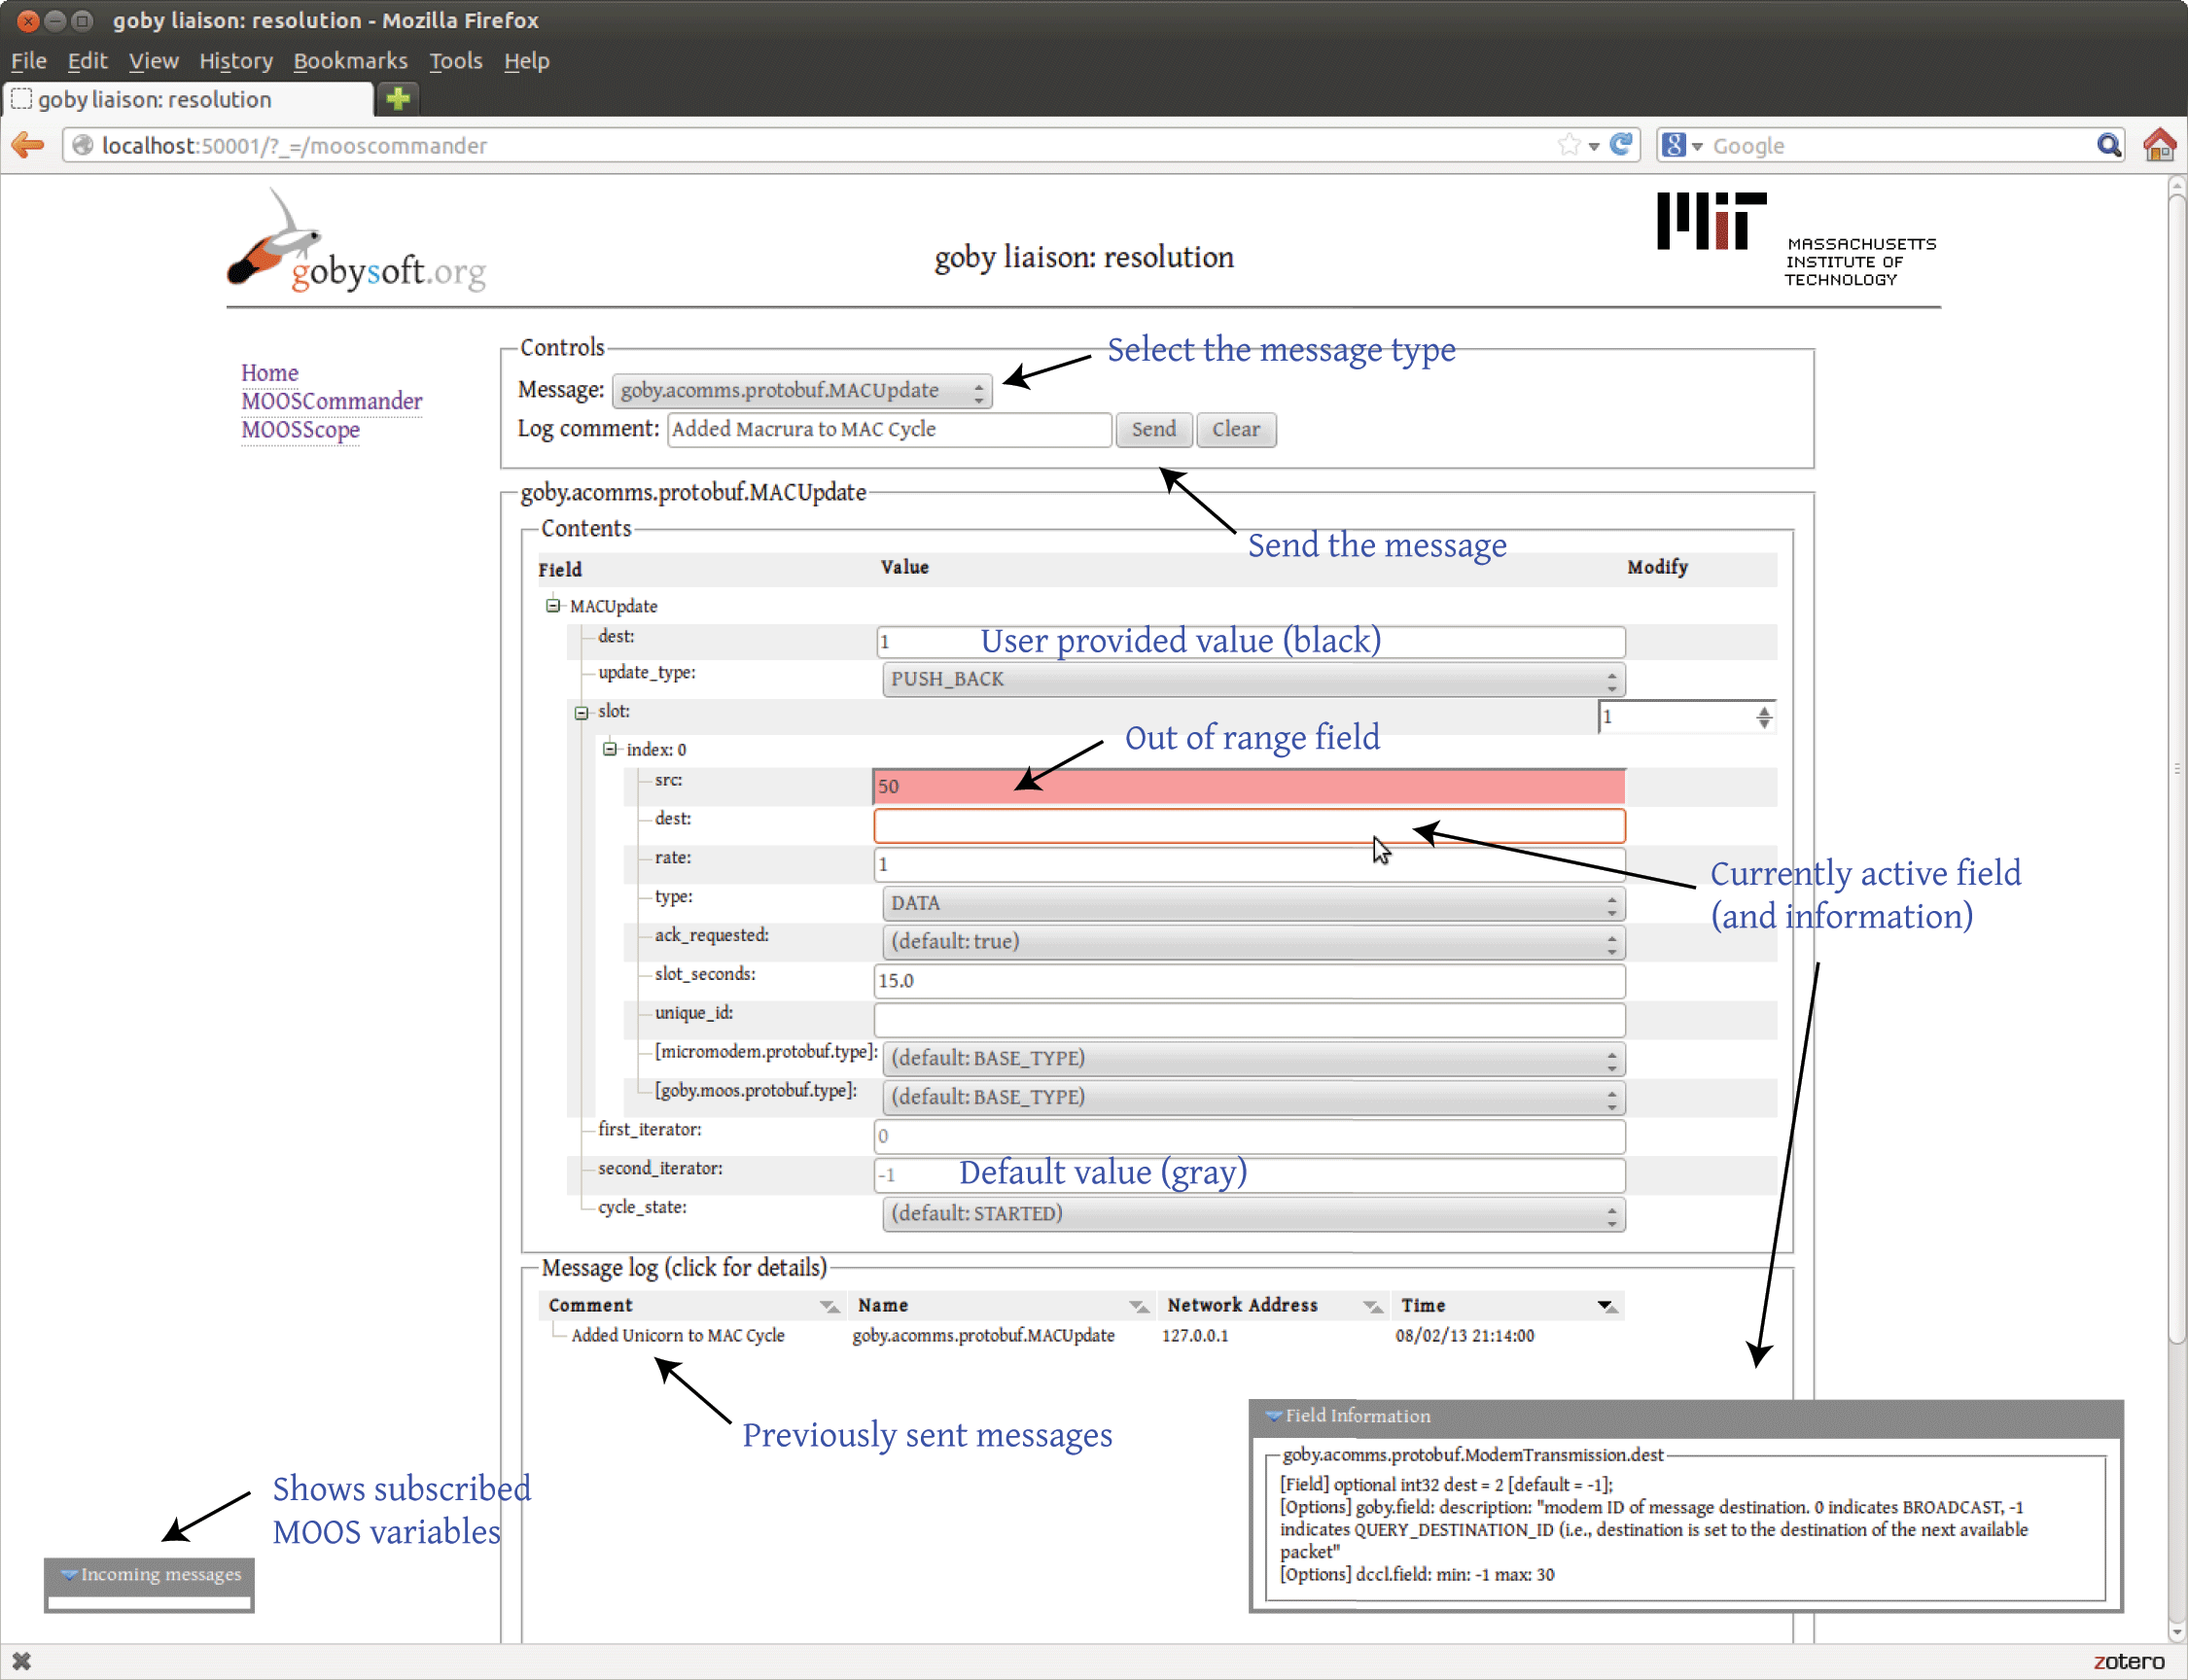
\includegraphics[width=7.5in, angle=90]{liaison_commander.png}
\caption{The MOOS Commander tab in Goby Liaison}
\label{fig:liaison_commander}
\end{figure}


The MOOS Commander tab is shown (with annotations) in Fig. \ref{fig:liaison_commander}. This is tool that allows a human operator to send DCCL messages (typically commands) to one or more robots. It supports sending any DCCL message (and any regular Protobuf message) known either at compile time  (!load_shared_library!) or runtime (!load_proto_file!).


When the MOOS plugins are loaded, the Commander tab can be configured with the following settings with the file passed to Liaison:

\boxedverbatiminput{@RELATIVE_CMAKE_CURRENT_SOURCE_DIR@/includes/moos_commander_liaison.pb.cfg}
\resetbvlinenumber


\begin{itemize}
\item !load_protobuf_name!: Repeated field, each with the full name of a Protobuf message as given by the !google::protobuf::Descriptor::full_name()!. This is the package name(s), followed by the message name, delimited by periods. For example, !example.MinimalStatus!. The messages will be loaded from !load_shared_library!, !load_proto_file!, and/or !load_proto_dir! configuration values given in the Liaison configuration, and made available for sending using the MOOS Commander GUI.
\item !value_width_pixels!: Change the display width of the !value! field (in pixels).
\item !modify_width_pixels!:  Change the display width of the !modify! field (in pixels).
\item !sqlite3_database!: Path to an SQLite3 database file to use (or create) to store all previously sent messages. Delete or modify this file to remove the history.
\item !database_pool_size!: The connection pool size for database connections. Generally this should be larger than the number of expected simultaneously connection clients to Liaison.
\item !database_view_height!: The height of the !Message log! section of the GUI (in pixels).
\item !database_width!: The widths (in pixels) of various components of the !Message log! section.
\item !modal_dimensions!:  The dimensions (in pixels) of the modal (popup) dialog when sending a message. 
\item !subscription!: A repeated field, each contains a MOOS variable name to subscribe for. Subscribed variables will be shown in the lower left corner of the Commander GUI.
\item !time_source_var!: The source of time e.g. !DB_TIME! from the MOOS database to be used for !codec="_time"! DCCL fields.
\end{itemize}


\subsection{MOOS Scope GUI (Liaison)}

\boxedverbatiminput{@RELATIVE_CMAKE_CURRENT_SOURCE_DIR@/includes/moos_scope_liaison.pb.cfg}
\resetbvlinenumber

\begin{itemize}
\item !subscription!: A repeated field, each with the string name of a MOOS variable. You can optionally use !*! at the end of the string for basic globbing. Use !regex_filter_expression! below for more advanced filtering. You can subscribe to !"*"! for all variables. Note that receiving mail for subscribed variables consumes network bandwidth, so it may be useful to subscribe to a small subset of variables before filtering when on a limited network connection.
\item !column_width!: Width (in pixels) for the individual scope columns.
\item !sort_by_column!: Which column to sort by on startup: Options are !COLUMN_KEY!, !COLUMN_TYPE!, !COLUMN_VALUE!, !COLUMN_TIME!, !COLUMN_COMMUNITY!, !COLUMN_SOURCE!, !COLUMN_SOURCE_AUX!, !COLUMN_MAX!.
\item !sort_ascending!: If true, sort ascending; if false, sort descending.
\item !scope_height!: Height (in pixels) of the scope display.
\item !regex_filter_column!: Which column to apply the !regex_filter_expression! to.
\item !regex_filter_expression!: A regular expression used to filter the scope results. Defaults to !".*"! which is an all-pass filter.
\item !history!: Enable one or more history panels showing the log of a given MOOS variable.
\begin{itemize}
\item !key!: The MOOS variable name to show history for.
\item !show_plot!: If true, shows a graph of the variable history. Only valid for MOOS double types.
\item !plot_width!: Width of the plot in pixels.
\item !plot_height!: Height of the plot in pixels.
\end{itemize}
\end{itemize}

\begin{figure}
\centering
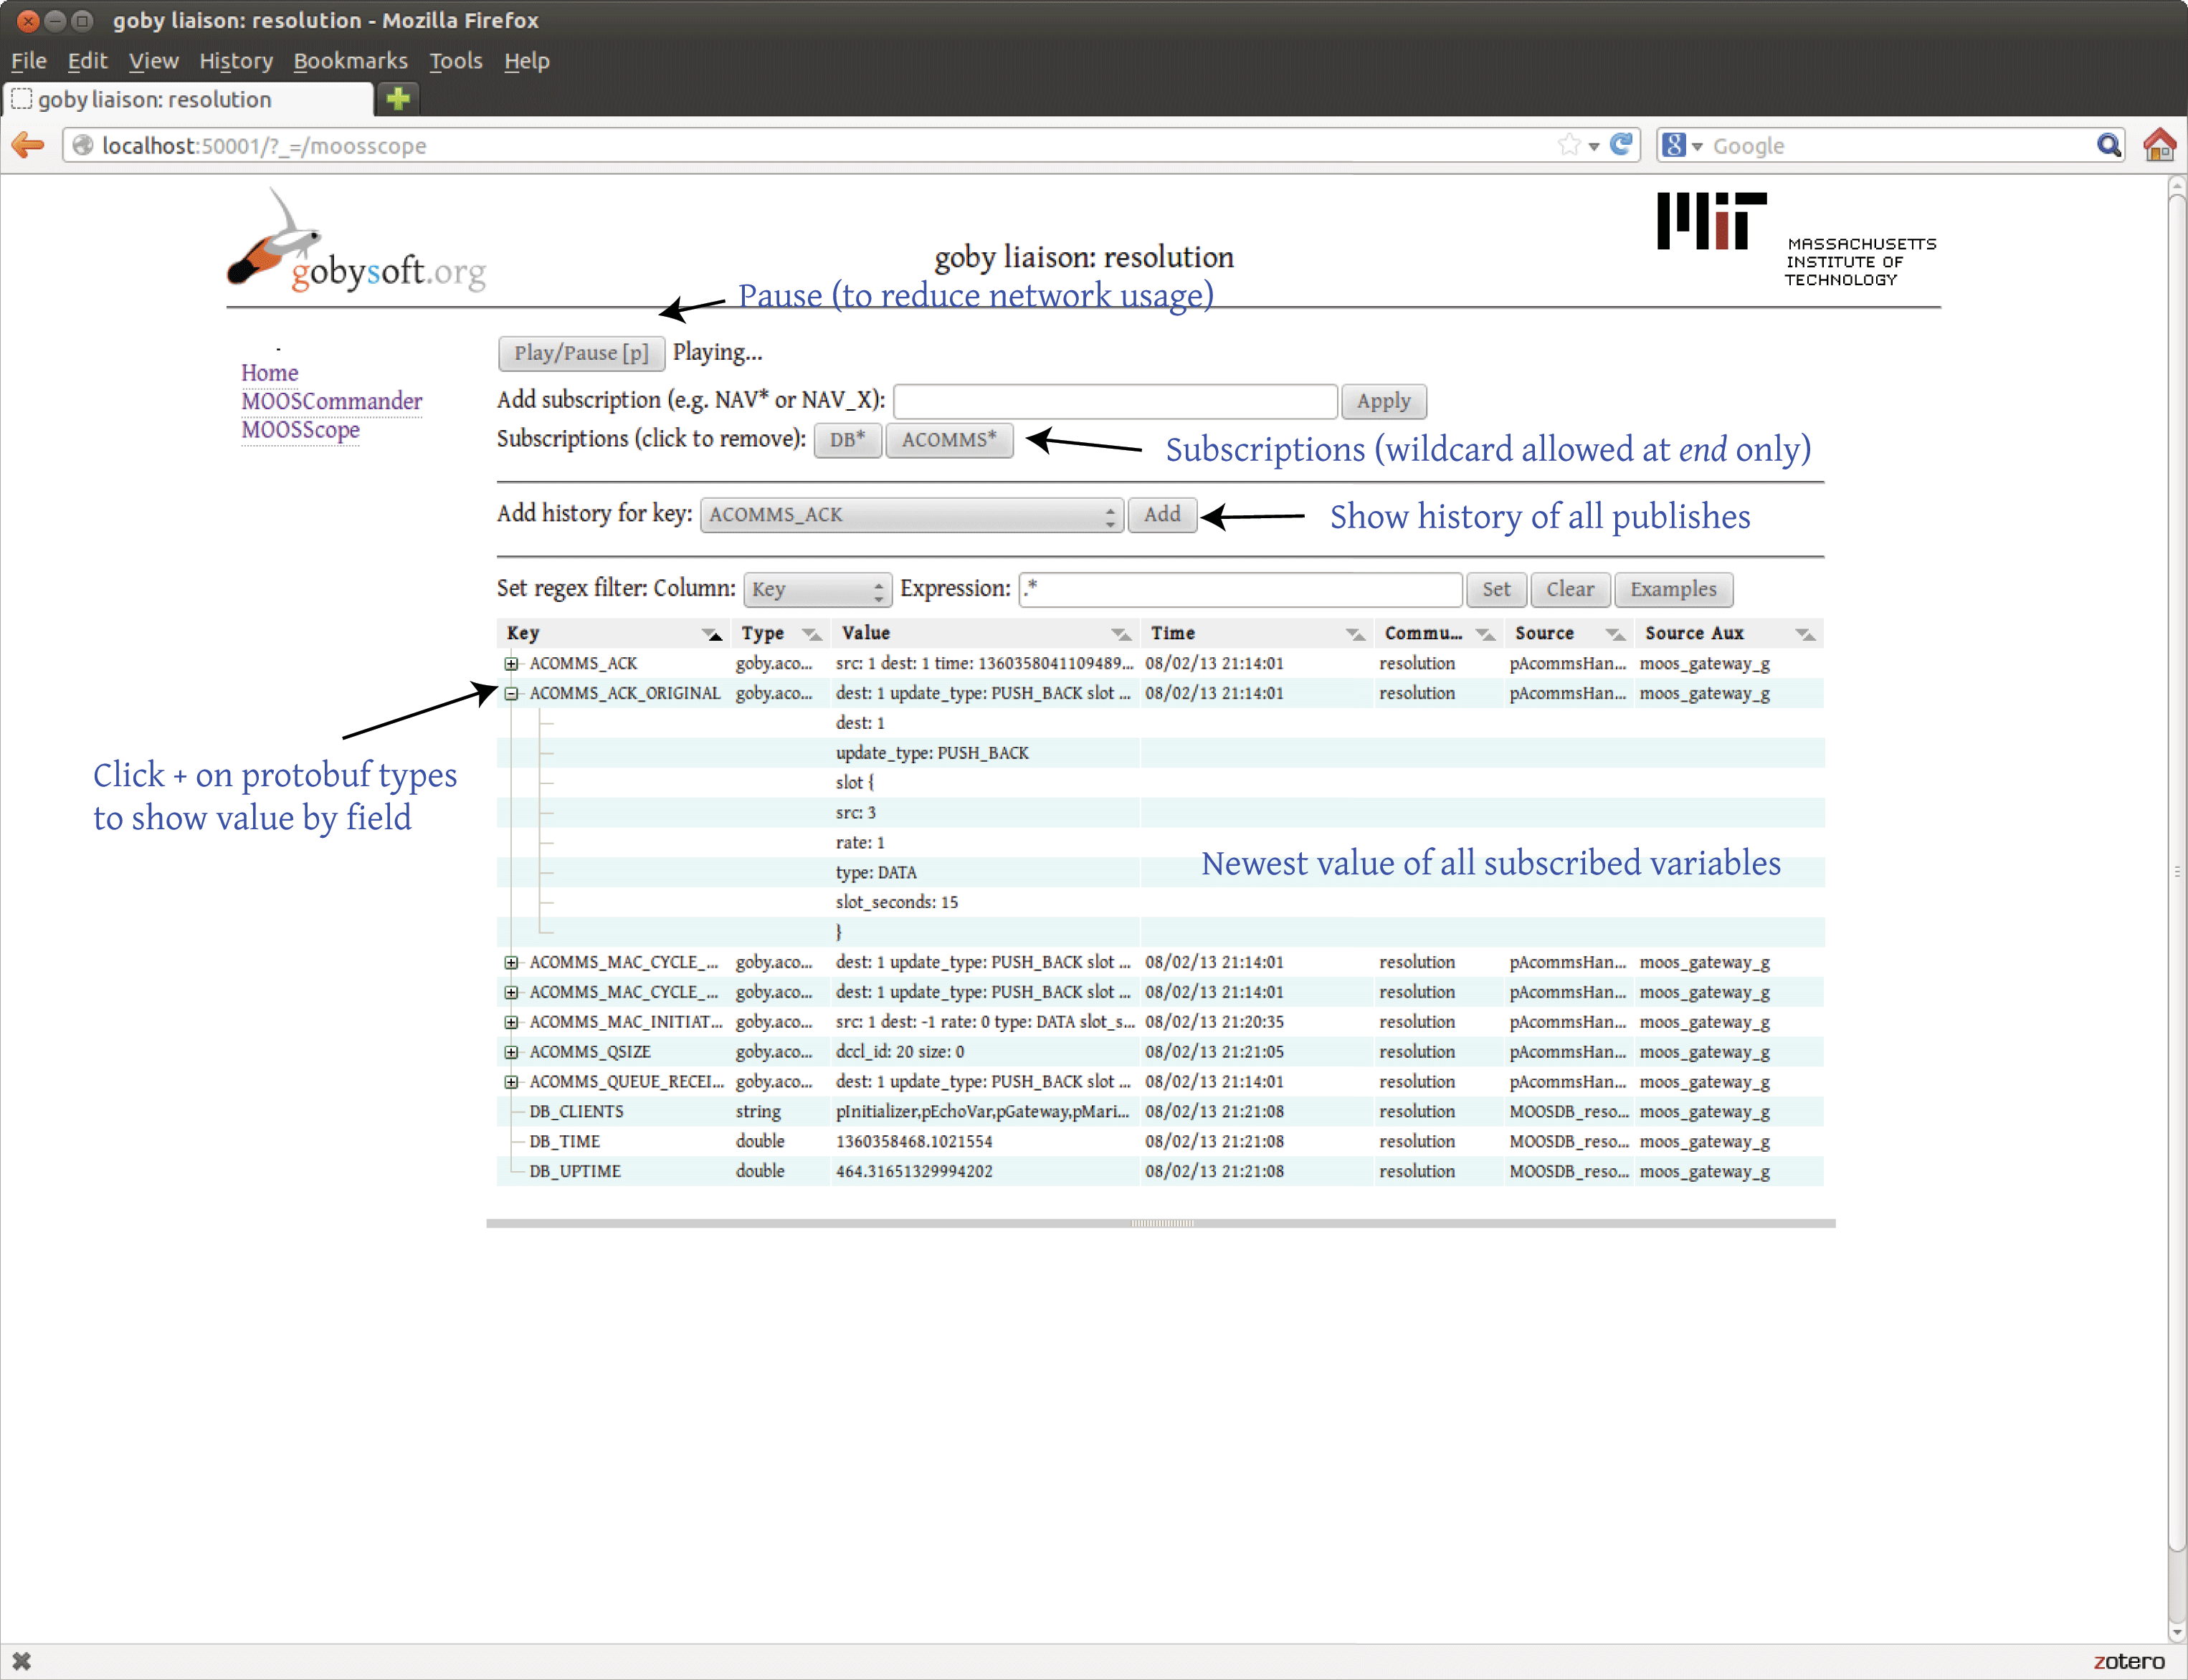
\includegraphics[width=7.5in, angle=90]{liaison_scope.png}
\caption{The MOOS Scope tab in Goby Liaison}
\label{fig:liaison_scope}
\end{figure}

\subsection{Example working configuration}

Here are the configuration files for !moos_gateway_g! and !goby_liaison! with the MOOS plugins enabled from a working system as an example:

\boxedverbatiminput{@RELATIVE_CMAKE_CURRENT_SOURCE_DIR@/includes/moos_gateway_g_ex1.pb.cfg}
\resetbvlinenumber

\boxedverbatiminput{@RELATIVE_CMAKE_CURRENT_SOURCE_DIR@/includes/goby_liaison_ex1.pb.cfg}
\resetbvlinenumber


\section{Migrating from Version 1 to Version 2} \label{sec:gobyv1_migrate}

pAcommsHandler from Goby version 2 (Goby2) provides nearly full backwards compatibility directly using the XML messages from Goby version 1 (Goby1). 

In order to use XML messages from Goby1 in Goby2, simply rename the !dccl_cfg! section of the pAcommsHandler1 configuration block to !transitional_cfg!. In general this is all that needs to be done, as pAcommsHandler2 will automatically internally convert the XML files to .proto files and load them. Some special features of the XML files are not supported in version 2:

\begin{itemize}
\item Algorithms without a corresponding source variable.
\item Algorithms with reference fields (e.g. subtract:timestamp) for message creation. Reference fields are still allowed upon publish.
\item \xmltag{format} tags must be specified in the boost::format !%1%!, !%2%!, etc. format, not using !%d! printf specifiers. The typed specifiers would work in Goby v1 but are not supported at all in Goby v2.
\end{itemize}

While the XML files can be used directly as a temporary measure, it is recommended to transition all your XML files to .proto files for direct use with pAcommsHandler2. To ease your transition, there is a tool !dccl_xml_to_dccl_proto! that will automatically convert your XML files for you. The usage is 
\begin{verbatim}
dccl_xml_to_dccl_proto message_xml_file.xml [directory for generated .proto (default = pwd (.)]
\end{verbatim}

In Goby1, the XML files contained both structure information and MOOS translation information. In Goby2, these are separated to allow better support of non-MOOS systems. 

The tool will write the generated .proto files (the structure information) to the directory specified as the second command line parameter (defaults to the current/working directory). It will write to standard output the required additions to the pAcommsHandler2 configuration file for the queuing and translation information present in the XML file. Simply copy these parts to your MOOS file and you can continue to use your old messages natively.


\section{iFrontSeat}
\label{sec:ifrontseat} 

\subsection{Introduction}

\subsubsection{Motivation}
Broadly, our goal in Goby is facilitate the development of a autonomy, sensing, and communications infrastructure that can operate on a heterogeneous collection of vehicles. One way to help effect this is to split the system into two components: the \textit{frontseat} and \textit{backseat} computing systems. The \textit{frontseat} is provided by the vehicle manufacturer and is typically proprietary. It is responsible for low level control of the vehicle. The \textit{backseat} runs the high level autonomy (typically the IvP Helm), sensing, and communications (typically Goby) components. The requirements of the \textit{frontseat} on the \textit{backseat} is minimally a continuous (e.g. 1 Hz) stream of course directives, such as desired heading, speed, and depth of the AUV. The requirements of the \textit{backseat} on the \textit{frontseat} is a best attempt to carry out these directives constrained by the dynamics of the vehicle, as well as a feed of the vehicles' navigation solution.

Not surprisingly, a piece of software is required to interface between the \textit{frontseat} and the \textit{backseat}. This code (!iFrontSeat!) is the subject of section.

Historically, a new interface has been written for each vehicle that was to be used with MOOS-IvP\footnote{For example, the applications iHuxley, iRecon, iOceanServerComms, $\ldots$}. This led to a proliferation of approaches for handling the state transitions and control, primarily from !pHelmIvP!. In some cases, misunderstandings involving various aspects of MOOS-IvP led to vehicle runaways. Furthermore, as MOOS-IvP becomes even more widely adopted and the number of manufacturers of robotic assets increases, it seems sensible to minimize the duplication of effort involved in writing interfaces.


\subsubsection{Design overview}

!iFrontSeat! (and its corresponding components in the library !libgoby_moos!) is comprised of two major components (the full UML structure diagram is given in Fig. \ref{fig:structure}):
\begin{itemize}
\item A base class !FrontSeatInterfaceBase! and MOOS Application !iFrontSeat! providing the IvP Helm state transition logic and MOOSDB subscriptions and publications. This is written \textit{once} and used by all the specific drivers. 
\item A collection of derived classes (which are compiled into individual shared libraries) to implement the interface provided by !FrontSeatInterfaceBase! for a given manufacturer or vehicle type. The currently available drivers include:
\begin{itemize}
\item !BluefinFrontSeat!: Implements !FrontSeatInterfaceBase! for the Bluefin Robotics family of AUVs using the Huxley software.
\end{itemize}
\end{itemize}

\begin{figure}
\centering
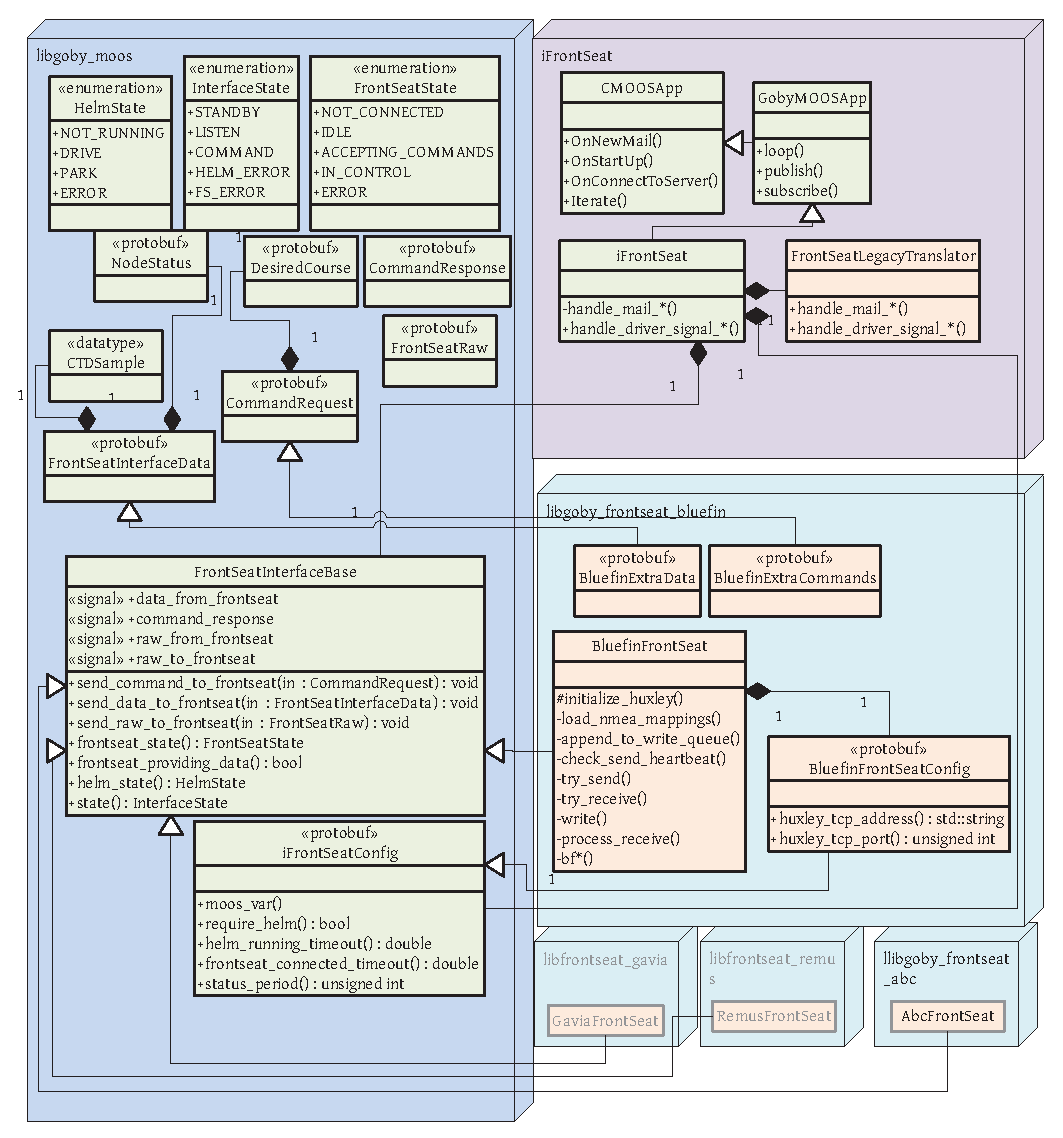
\includegraphics[width=\textwidth]{iFrontSeat_structure.eps}
\caption{Structure diagram of iFrontSeat and supporting libraries. Green components are implemented once and used by all the drivers (see Chapter \ref{chap:common}). Pink components need to be modified/implemented for each specific driver (see Chapter \ref{chap:specific}).}
\label{fig:structure}
\end{figure}

\subsubsection{Running iFrontSeat}

iFrontSeat always requires exactly one driver library to be loaded before any command-line parameters will be accepted. The driver libraries are runtime-loaded because this allows for a driver developer to create his or her own driver without changing any of the Goby source code. The driver library is loaded from the environmental variable !IFRONTSEAT_DRIVER_LIBRARY!. For example, use the bash shell, one can load iFrontSeat with the Bluefin driver (see section \ref{sec:bluefin_specific}) with this invocation:

\begin{verbatim}
IFRONTSEAT_DRIVER_LIBRARY=libgoby_frontseat_bluefin.so.25 iFrontSeat 
\end{verbatim}

The library specified must be a complete path or on the !ld! library search path (e.g. set using !LD_LIBRARY_PATH!). Alternatively, you could export !IFRONTSEAT_DRIVER_LIBRARY! from one of the shell configuration files (e.g. !~/.bashrc!), and then simply run !iFrontSeat! on the command line. 

\subsection{Shared MOOS Side Components}\label{chap:common}

iFrontSeat is a Goby MOOS application, which means it uses a validating configuration reader based on Google Protocol Buffers instead of the standard MOOS ProcessConfigReader. The syntax is similar, and you can always get all the valid configuration parameters by running
\begin{verbatim}
iFrontSeat --example_config
\end{verbatim}

Many of these parameters can be left to their defaults, except for special cases and advanced usages. 

This was the configuration of iFrontSeat at the time of writing this technical report. Be sure to check !iFrontSeat --example_config! for the latest possible valid configuration.

\begin{boxedverbatim}
ProcessConfig = iFrontSeat
{
  common {
	// configuration common to all Goby Applications	
	// ...
    }
  }
  require_helm: true
  helm_running_timeout: 10
  frontseat_connected_timeout: 10
  status_period: 5
  moos_var {
    prefix: "IFS_" 
    raw_out: "RAW_OUT"
    raw_in: "RAW_IN"
    command_request: "COMMAND_REQUEST"
    command_response: "COMMAND_RESPONSE"
    data_from_frontseat: "DATA_IN"
    data_to_frontseat: "DATA_OUT"
    status: "STATUS"
  }
  exit_on_error: false
  legacy_cfg {
    subscribe_desired: true
    subscribe_ctd: false
    subscribe_acomms_raw: false
    pub_sub_bf_commands: false
    publish_nav: true
    publish_fs_bs_ready: false
  }

  // vehicle driver specific configuration
  // ... 
}
\end{boxedverbatim}
\resetbvlinenumber

The configuration for iFrontSeat has three main parts:
\begin{enumerate}
\item The !common! configuration which is the same for all Goby MOOS applications. Please see section \ref{sec:goby_moos_app} for details. Setting !verbosity: DEBUG2! is useful for debugging (and also !show_gui: true!, which displays an NCurses screen with useful debugging information). 
\item The configuration for the shared MOOS side components, described below in this section.
\item The vehicle driver specific configuration, described in Chapter \ref{chap:specific}.
\end{enumerate}

The configuration for the shared MOOS components is:

\begin{itemize}
\item !require_helm!: Require the IvP Helm even for a listening mission where the frontseat is in control (default=true).
\item !helm_running_timeout!:  If !require_helm: true!, how long (in seconds) to wait for the IvP Helm to start before moving to the Helm Error state. (default=10)
\item !frontseat_connected_timeout!: How long (in seconds) to wait for the Frontseat to be connected before moving to the Frontseat Error state. (default=10)
\item !status_period!: Seconds between publishing the status of iFrontseat. The special value 0 disables posting of the status message (default=5).
\item !moos_var!: Change the default values of the MOOS variables published or subscribed to by iFrontSeat. Throughout the manual, these defaults are referenced. If you change the values here, keep this in mind when reading the rest of the manual.
\begin{itemize}
\item !prefix!: Prefix all MOOS variable names with this string (default=``IFS\_'')
\item !raw_out!: (default=``RAW\_OUT'')
\item !raw_in!: (default=``RAW\_IN'')
\item !command_request!: (default=``COMMAND\_REQUEST'')
\item !command_response!: (default=``COMMAND\_RESPONSE'')
\item !data_from_frontseat!: (default=``DATA\_IN'')
\item !data_to_frontseat!: (default=``DATA\_OUT'')
\item !status!: "STATUS" (default=``STATUS'')
\end{itemize}  
\item !exit_on_error!: If true, exit the application if it enters one of the error states. Use only for debugging. (default=false)
\item !legacy_cfg!: Numerous options to automatically convert legacy variables (e.g., from iHuxley) into the iFrontSeat messages. Generally new projects will not use any of these options and thus this configuration block can be omitted. See section \ref{sec:ifrontseat_legacy_cfg} for details on which of these flags to enable if legacy compatibility is desired.
\end{itemize}

\subsubsection{MOOS Variable Interface}

The preferred way to use iFrontSeat is via the new !IFS_! set of variables. The contents of these string MOOS variables are the output of the !TECHNIQUE_PREFIXED_PROTOBUF_TEXT_FORMAT! translator explained in the Goby2 user manual (\url{http://gobysoft.com/dl/goby2-user-manual.pdf}). Essentially, they are the !TextFormat! human-readable output of the Google Protocol Buffers messages defined in
\begin{verbatim}
goby/moos/protobuf/frontseat.proto
\end{verbatim}

To get access to the C++ equivalent classes generated by the Protobuf C++ compiler (protoc), include this header:
\begin{verbatim}
#include "goby/moos/protobuf/frontseat.pb.h"
\end{verbatim}

Do not parse these messages manually. You can automatically parse and serialize these values to and from the corresponding Protobuf C++ classes using the functions !serialize_for_moos! and !parse_for_moos!, which are declared in the header file:
\begin{verbatim}
#include "goby/moos/moos_protobuf_helpers.h" 
\end{verbatim}

The MOOS variables \textbf{subscribed} to by iFrontSeat include (note the names are configurable, the defaults are given here):
\begin{itemize}
\item !IFS_COMMAND_REQUEST!: Command from to give to the frontseat driver to be asked of the vehicle's computer. This is typically the desired course (heading, speed, and depth) of the vehicle. Other special commands may be defined by the specific vehicle driver. Protobuf Message type:  !CommandRequest!.
\item !IFS_DATA_TO_FRONTSEAT!: Data that must be passed to the frontseat driver. For example, the Bluefin AUVs require Conductivity-Temperature-Depth (CTD) measurements when the CTD is connected to the backseat computer. Protobuf Message type: !goby.moos.protobuf.FrontSeatInterfaceData!.
\end{itemize}

The MOOS variables \textbf{published} by iFrontSeat include:
\begin{itemize}
\item !IFS_COMMAND_RESPONSE!: Response to each command request, if a response is requested. Protobuf Message type:  !goby.moos.protobuf.CommandResponse!.
\item !IFS_STATUS!: The current state of the IvP Helm, the frontseat system, and the interface itself. Protobuf Message type:  !goby.moos.protobuf.FrontSeatInterfaceStatus!.
\item !IFS_DATA_FROM_FRONTSEAT!: Data from the frontseat driver. This may include navigation data (vehicle's current pose, speed, depth, latitude, longitude, etc), or other vehicle specific data. Protobuf Message type: !goby.moos.protobuf.FrontSeatInterfaceData!.
\item !IFS_RAW_IN!: Raw communications packets (e.g. NMEA-0183) from the frontseat computer to iFrontSeat. Protobuf Message type: !goby.moos.protobuf.FrontSeatRaw!
\item !IFS_RAW_OUT!: Raw communications packets (e.g. NMEA-0183) from iFrontSeat to the frontseat computer. Protobuf Message type: !goby.moos.protobuf.FrontSeatRaw! 
\end{itemize}

\subsubsection{Legacy MOOS Variable Interface}\label{sec:ifrontseat_legacy_cfg}

iFrontSeat aims to replace several existing pieces of software, and by necessity provides a number of features to ease transition. This functionality may change or be removed in future versions, so where possible please use the new !IFS_! variables. This legacy functionality is implemented in:

\begin{verbatim}
goby/src/apps/moos/iFrontSeat/legacy_translator.cpp
goby/src/apps/moos/iFrontSeat/legacy_translator.h
\end{verbatim}

The transitional MOOS variables \textbf{subscribed} to by iFrontSeat include:

\begin{itemize}
\item If !subscribe_ctd: true!, then !CTD_CONDUCTIVITY! (siemens/meter), !CTD_TEMPERATURE! (degrees C), !CTD_PRESSURE! (decibars), !CTD_SALINITY! (unitless - practical salinity scale). These double values are buffered, then upon receipt of !CTD_TEMPERATURE! are converted into a !FrontSeatInterfaceData! message containing a !CTDSample! and published to !IFS_DATA_TO_FRONTSEAT!.
\item If !subscribe_desired: true!, then !DESIRED_HEADING! (degrees), !DESIRED_SPEED! (meters/second), !DESIRED_DEPTH! (meters). These desired course values (typically published by pHelmIvP) are buffered and upon receipt of !DESIRED_SPEED! are converted to a !CommandRequest! and posted to !IFS_COMMAND_REQUEST!.
\item If !pub_sub_bf_commands: true!, then !PENDING_SURFACE!: This double value posted by BHV\_PeriodicSurface creates a !CommandRequest! of the special Bluefin type: !BluefinExtraCommands::GPS_REQUEST!. This allows the shallow water vehicles that require a GPS fix to occasionally come to the surface for GPS.
\item If !subscribe_acomms_raw: true!, then !ACOMMS_RAW_INCOMING!, !ACOMMS_RAW_OUTGOING!: The raw NMEA-0183 feed from the WHOI Micro-Modem (or other acoustic modem) posted by the Goby-Acomms MOOS application pAcommsHandler. These are converted into a !FrontSeatInterfaceData! message containing the special Bluefin extension !BluefinExtraData.micro_modem_raw_in! or !BluefinExtraData.micro_modem_raw_out! and published to !IFS_DATA_TO_FRONTSEAT!. Bluefin still requires our raw Micro-Modem feed as a backup to the hardware tail-cone abort (which uses the Micro-Modem). 
\end{itemize}

The transitional MOOS variables \textbf{published} by iFrontSeat include:

\begin{itemize}
\item If !publish_nav: true!, then !NAV_X! (meters), !NAV_Y! (meters), !NAV_LAT! (degrees), !NAV_LONG! (degrees), !NAV_Z! (meters, negative down), !NAV_DEPTH! (meters, positive down), !NAV_YAW! (degrees), !NAV_HEADING! (degrees), !NAV_SPEED! (meters/second), !NAV_PITCH! (radians), !NAV_ROLL! (radians), !NAV_ALTITUDE! (meters). All these double values are generated from the !FrontSeatInterfaceData! message when it contains !node_status! information.
\item If !publish_fs_bs_ready: true!, then !BACKSEAT_READY!: Published as 1 (true) when the Helm State becomes !HELM_DRIVE!, otherwise 0 (false).
\item If !publish_fs_bs_ready: true!, then !FRONTSEAT_READY!: Published as 1 (true) when the FrontSeat State becomes !FRONTSEAT_ACCEPTING_COMMANDS!, otherwise 0 (false).
\item !GPS_UPDATE_RECEIVED!: Published as !Timestamp=double seconds since Unix! when a !BluefinExtraCommands::GPS_REQUEST! command responds successfully.
\end{itemize}

\subsection{Vehicle Drivers}\label{chap:specific}

\subsubsection{BluefinFrontSeat}\label{sec:bluefin_specific}

The driver !BluefinFrontSeat! is designed for the Bluefin Robotics Standard Payload Interface (SPI) Version 1.8 and newer, which must be requested directly from Bluefin Robotics. 

Knowledge of some details of Bluefin's SPI will be assumed here; please reference that document as needed while reading this section.

The configuration accepted by iFrontSeat for the !BluefinFrontSeat! driver is as follows:

\begin{boxedverbatim}

  [bluefin_config] { 
    huxley_tcp_address: "" 
    huxley_tcp_port: 29500 
    reconnect_interval: 10 
    nmea_resend_attempts: 3 
    nmea_resend_interval: 5 
    allowed_nmea_demerits: 3 
    allow_missing_nav_interval: 5 
    heartbeat_interval: 1  
    extra_bplog: ""  
    send_tmr_messages: true
    disable_ack: false
    accepting_commands_hook: BFMSC_TRIGGER 
  }
\end{boxedverbatim}
\resetbvlinenumber

This configuration values are placed in the .moos file in the !ProcessConfig = iFrontSeat! block:

\begin{itemize}
\item !huxley_tcp_address!: IP address or domain name of the Huxley server machine.
\item !huxley_tcp_port!: TCP port of the Huxley server. (default=29500)
\item !reconnect_interval!: How many seconds to wait between reconnects if the Huxley server disconnects. (default=10)
\item !nmea_resend_attempts!: Number of resend attempts for a given NMEA message (default=3)
\item !nmea_resend_interval!: How many seconds to wait between resend attempts (default=5)
\item !allowed_nmea_demerits!: Number of times Huxley can fail to acknowledge a NMEA message before we close the connection. (default=3)
\item !allow_missing_nav_interval!: How many seconds to allow without !$BFNVG! before declaring frontseat not providing us data. (default=5)
\item !heartbeat_interval!:  How many seconds between heartbeats (!$BPSTS!). (default=1)
\item !extra_bplog!: Additional Bluefin messages to enable logging for (e.g. for to send !$BPLOG,CMA,ON!, set this field to 'CMA'. This field can be repeated.
\item !send_tmr_messages!: Send the BPTMR message with acoustic comms contents. This is required on certain vehicles outfitted with the WHOI Micro-Modem. Ask Bluefin for details about if they need the BPTMR message sent (default=true). %$
\item !disable_ack!: If true, do not use the BFACK message. Set to true for vehicles without the BFACK support. Note that if this field is set to true, !IFS_COMMAND_RESPONSE! messages will not be posted.
\item !accepting_commands_hook!: The mechanism by which the Bluefin frontseat indicates that it is ready to accept commands from iFrontSeat (and also by which it revokes control). The options are:
\begin{itemize}
\item !BFMSC_TRIGGER!: If any BFMSC message is received, the frontseat state is set to !FRONTSEAT_ACCEPTING_COMMANDS!. If a BFMIS message is received with the word ``Running'' in the fourth field, the frontseat state is set to be !FRONTSEAT_IN_CONTROL!. Any other BFMIS sets the frontseat state to !FRONTSEAT_IDLE!.
\item !BFMIS_RUNNING_TRIGGER!: If a BFMIS message is received with the word ``Running'' in the fourth field, the frontseat state is set to be !FRONTSEAT_ACCEPTING_COMMANDS!.  Any other BFMIS sets the frontseat state to !FRONTSEAT_IDLE!.
\item !BFCTL_TRIGGER!: If the third field is true, the frontseat state is set to !FRONTSEAT_ACCEPTING_COMMANDS!. Otherwise, it is set to !FRONTSEAT_IN_CONTROL!. Also, if a BFMIS message is received with the word ``Running'' in the fourth field, the frontseat state is set to be !FRONTSEAT_IN_CONTROL!.  Any other BFMIS sets the frontseat state to !FRONTSEAT_IDLE!.
\end{itemize} 
\end{itemize}


\subsubsection{Writing a new driver}



\section{iCommander}\label{sec:icommander} 

\textit{Deprecated. Use goby\_liaison as a replacement. See section \ref{sec:moos_liaison}.}

\section{pREMUSCodec}

\textit{Deprecated, see section \ref{sec:ccl_dccl_example} for an example of using pAcommsHandler with CCL.}

\DeleteShortVerb{\!}
